%====================================================================================
\chapter{Modelo de interacción con el usuario}
\label{cap:reqSist}

%====================================================================================
%Interfaces del Modulo de Control Acceso.
%=============================================================================

\section{Interfaces del subsistema: Control acceso}

\subsection{CU01 Resgistro de usuario}
{
\justify
\color{blue}{\textbf{Objetivo}}
}

%------------------------------------------------------------------
\justify
En esta pantalla permite al usuario registrar sus datos para crear una cuenta en el sistema.
%------------------------------------------------------------------
{
\justify
\color{blue}{\textbf{	Diseño}}
}
%-------------------------------------------------------------------------------
\justify
En la figura 8.1 se muestra a pantalla, en donde el usuario registra sus datos.

\begin{figure}[htb]
\centering
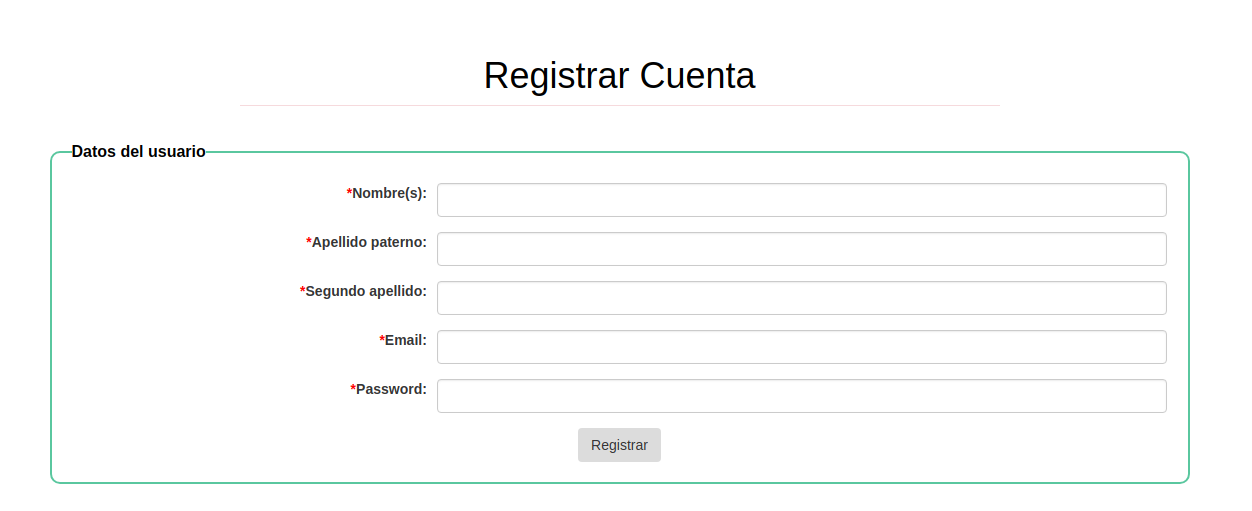
\includegraphics[width=0.8\textwidth]{./images/cu01-registro-usuario.png}
\caption{Registro de usuario.} \label{fig:IU01}
\end{figure}
%===================================================================================
\subsection{CU02 Login}
{
\justify
\color{blue}{\textbf{Objetivo}}
}
%------------------------------------------------------------------
\justify
En esta pantalla permite al usuario iniciar sesión en el sistema.
%------------------------------------------------------------------
{
\justify
\color{blue}{\textbf{Diseño}}
}
%-------------------------------------------------------------------------------
\justify
En la figura 8.2 se muestra a pantalla, en donde el usuario introducira los parametros necesarios para accceder al sistema.

\begin{figure}[htb]
\centering
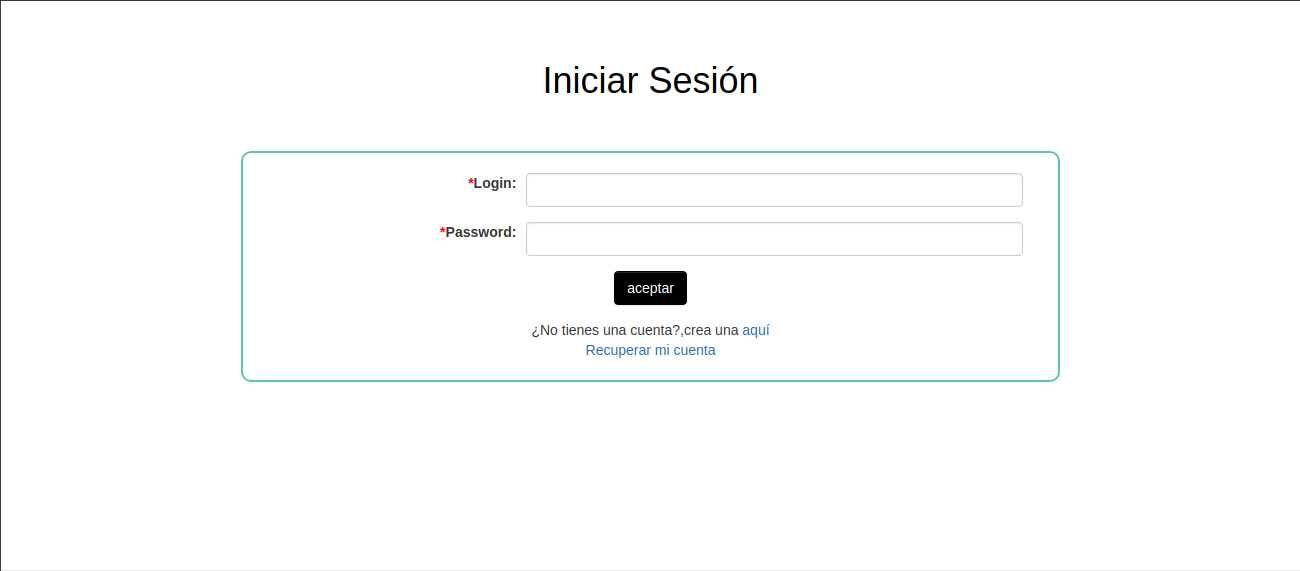
\includegraphics[width=0.8\textwidth]{./images/cu02-login.png}
\caption{Login.} \label{fig:horizonte}
\end{figure}
%===================================================================================
\subsection{CU08 Recuperar contraseña}
{
\justify
\color{blue}{\textbf{Objetivo}}
}
%------------------------------------------------------------------
\justify
En esta pantalla permite al usuario recuperar su contraseña en caso de no recordarla.
%------------------------------------------------------------------
{
\justify
\color{blue}{\textbf{Diseño}}
}
%-------------------------------------------------------------------------------
\justify
En la figura 8.3 se muestra a pantalla, en donde el usuario introducira su correo electronico para reuperar su contraseña.

\begin{figure}[htb]
\centering
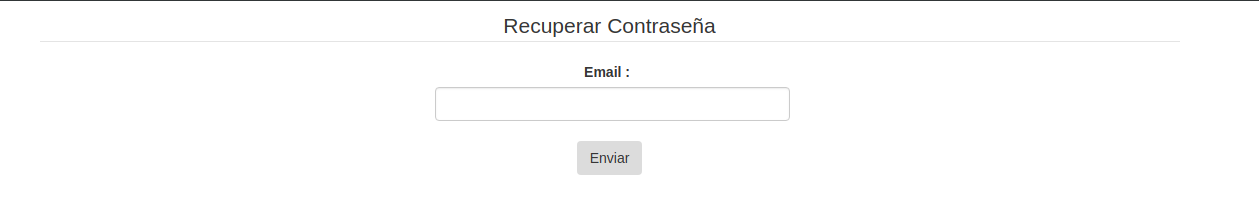
\includegraphics[width=0.8\textwidth]{./images/cu03-recuperar-contrasena.png}
\caption{Recuerar contraseña.} \label{fig:horizonte}
\end{figure}
%===================================================================================
\subsection{CU15 Cambiar Contraseña}
{
\justify
\color{blue}{\textbf{Objetivo}}
}

%------------------------------------------------------------------
\justify
En esta pantalla permite al usuario modificar la contraseña de su cuenta.
%------------------------------------------------------------------
{
\justify
\color{blue}{\textbf{Diseño}}
}
%-------------------------------------------------------------------------------
\justify
En la figura \ref{fig:IU15} se muestra a pantalla, en donde el usuario registra sus datos.

\begin{figure}[htb]
\centering

\includegraphics[width=0.8\textwidth]{./images/cu15-cambiar-contrasena.png}
\caption{Cambiar contraseña.} \label{fig:IU15}
\end{figure}
%Interfaces del Modulo de Gesitión de Proyectos
%==================================================================================
%=============================================================================

\section{Interfaces del subsistema: Gestión de proyectos}

\subsection{CU03 Crear Proyecto}
{
\justify
\color{blue}{\textbf{Objetivo}}
}

%------------------------------------------------------------------
\justify
En esta pantalla permite al Lider de proyecto crear un proyecto.
%------------------------------------------------------------------
{
\justify
\color{blue}{\textbf{Diseño}}
}
%-------------------------------------------------------------------------------
\justify
En la figura \ref{fig:IU03} se muestra la pantalla, en donde el Lider de proyecto introducira los parametros necesarios para registrar un proyecto.

\begin{figure}[htb]
\centering
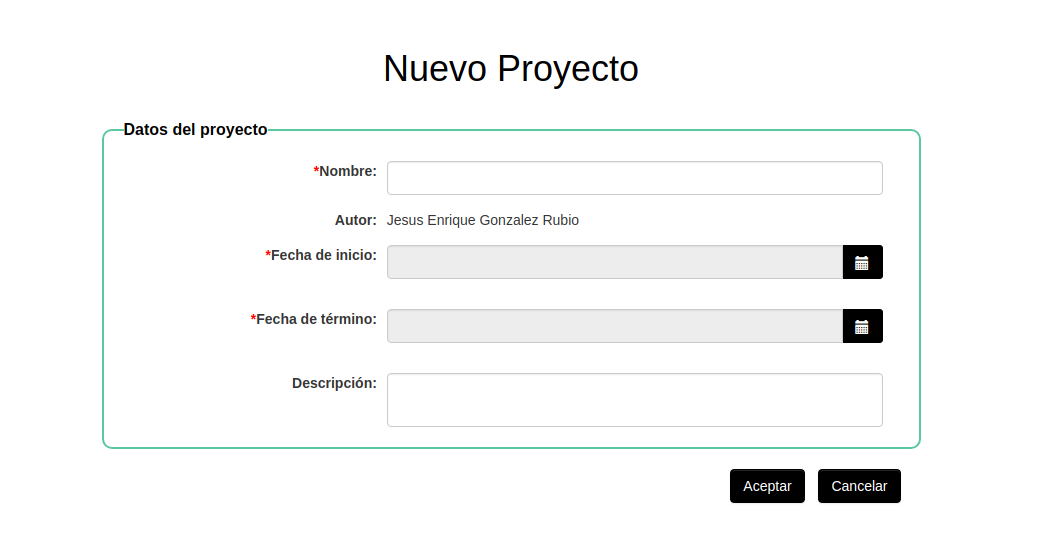
\includegraphics[width=0.8\textwidth]{./images/cu03-crear-proyecto.png}
\caption{Crear proyecto.} \label{fig:IU03}
\end{figure}
%===================================================================================
\subsection{CU16 Editar Proyecto}
{
\justify
\color{blue}{\textbf{Objetivo}}
}

%------------------------------------------------------------------
\justify
En esta pantalla permite al Lider proyecto editar los parametros de configuracin del proyecto.
%------------------------------------------------------------------
{
\justify
\color{blue}{\textbf{Diseño}}
}
%-------------------------------------------------------------------------------
\justify
En la figura \ref{fig:IU16} se muestra a pantalla, en donde el Lider de proyecto editara los parametros de configuracion del proyecto.

\begin{figure}[htb]
\centering
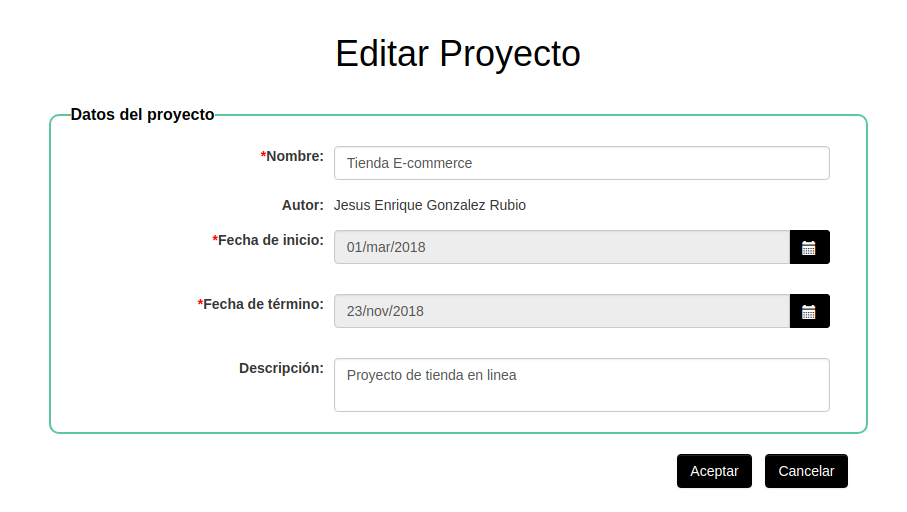
\includegraphics[width=0.8\textwidth]{./images/cu16-editar-proyecto.png}
\caption{Editar Proyecto.} \label{fig:IU16}
\end{figure}
%===================================================================================
\subsection{CU17 Información del proyecto}
{
\justify
\color{blue}{\textbf{Objetivo}}
}

%------------------------------------------------------------------
\justify
En esta pantalla permite al Lider proyecto podra ver los datos generales del proyecto.
%------------------------------------------------------------------
{
\justify
\color{blue}{\textbf{Diseño}}
}
%-------------------------------------------------------------------------------
\justify
En la figura \ref{fig:IU17} se muestra la pantalla, en donde el Lider de proyecto podrá ver los datos generales del proyecto.

\begin{figure}[htb]
\centering
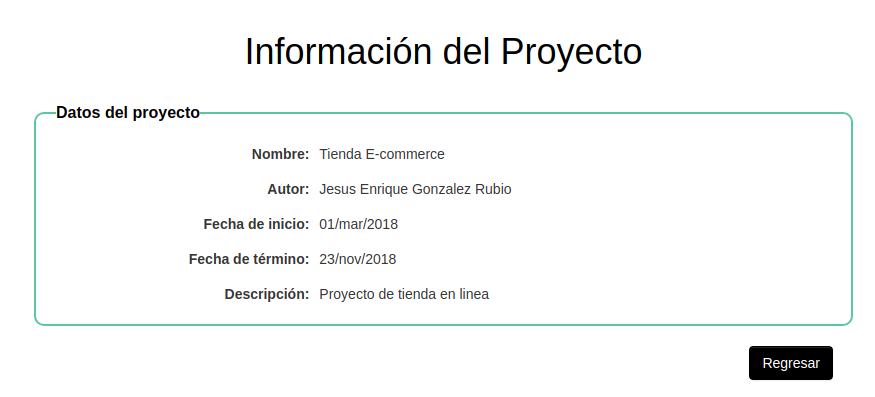
\includegraphics[width=0.8\textwidth]{./images/cu17-informacion-proyecto.png}
\caption{Editar Proyecto.} \label{fig:IU17}
\end{figure}
%===================================================================================
\subsection{CU19 Registrar repositorio proyecto}
{
\justify
\color{blue}{\textbf{Objetivo}}
}

%------------------------------------------------------------------
\justify
En esta pantalla permite al Lider proyecto registrar el repositorio en donde se esta versionando el proyecto.
%------------------------------------------------------------------
{
\justify
\color{blue}{\textbf{Diseño}}
}
%-------------------------------------------------------------------------------
\justify
En la figura \ref{fig:IU19} se muestra la pantalla, en donde el Lider de proyecto podrá registrar el repositorio en donde se esta versionando el proyecto.

\begin{figure}[htb]
\centering
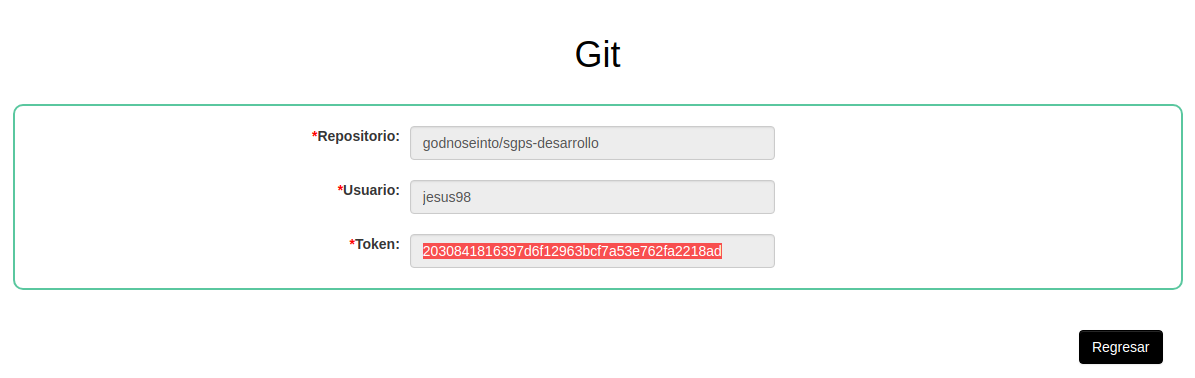
\includegraphics[width=0.8\textwidth]{./images/cu19-registrar-repositorio-proyecto.png}
\caption{Registrar repositorio proyecto.} \label{fig:IU19}
\end{figure}
%Interfaces del Modulo de Gestión de tareas
%===================================================================================
\section{Interfaces del subsistema: Gestión de tareas}

\subsection{CU20 Configuración de tareas}
{
\justify
\color{blue}{\textbf{Objetivo}}
}

%------------------------------------------------------------------
\justify
Permite al Lider de proyecto configurar las tareas que se realizaranen el proyecto, poder visuizaras en un diagrama de gantt y gestionar los avances atraves de un diagrama de representacion de avances por tareas.
%------------------------------------------------------------------
{
\justify
\color{blue}{\textbf{Diseño}}
}
%-------------------------------------------------------------------------------
\justify
En la figura \ref{fig:IU20} se muestra la pantalla, en donde permíte al Lider de proyecto configurar las tareas que se realizaranen el proyecto, poder visuizaras en un diagrama de gantt y gestionar los avances atraves de un diagrama de representacion de avances por tareas.

\begin{figure}[htb]
\centering
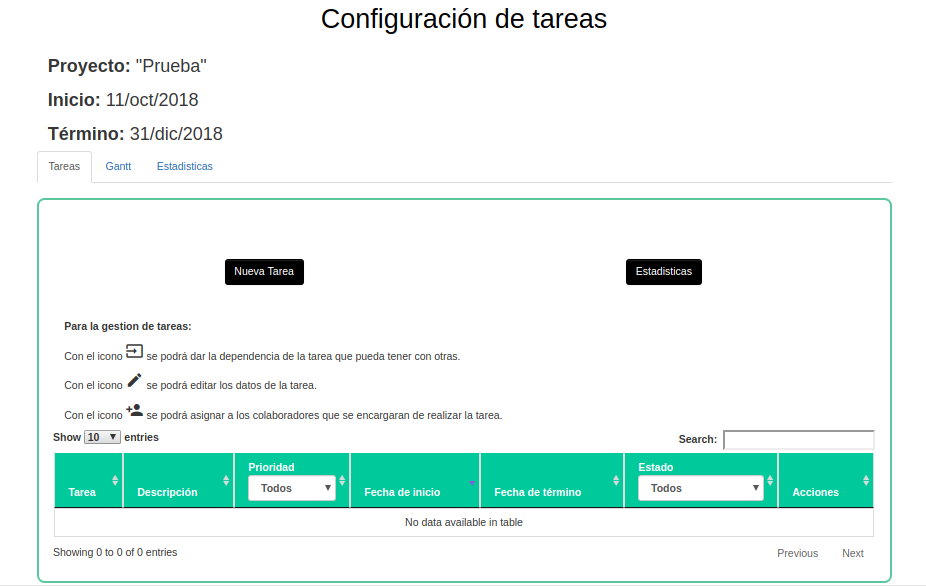
\includegraphics[width=0.8\textwidth]{./images/cu20-configurar-tareas.png}
\caption{Configuración de tareas.} \label{fig:IU20}
\end{figure}
%===================================================================================
\subsection{CU21 Relacionar tareas}
{
\justify
\color{blue}{\textbf{Objetivo}}
}

%------------------------------------------------------------------
\justify
Permite al Lider de proyecto relacionar las tareas que esten configuradas en el sistema.
%------------------------------------------------------------------
{
\justify
\color{blue}{\textbf{Diseño}}
}
%-------------------------------------------------------------------------------
\justify
En la figura \ref{fig:IU21} se muestra la pantalla, en donde permite al Lider de proyecto relacionar las tareas que esten configuradas en el sistema.

\begin{figure}[htb]
\centering
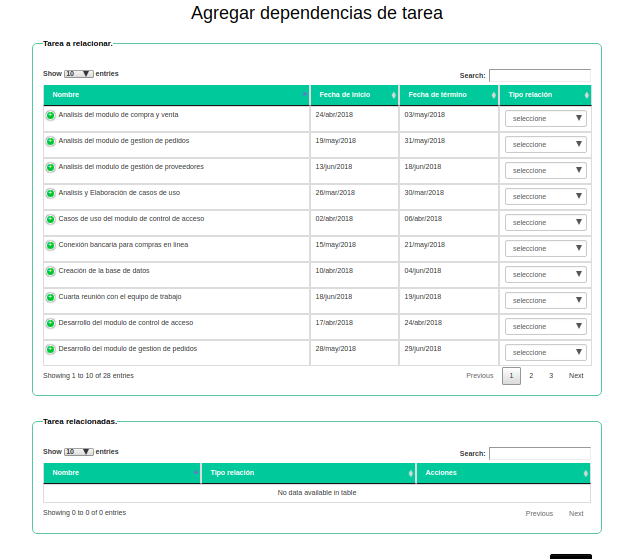
\includegraphics[width=0.8\textwidth]{./images/cu21-relacionar-tareas.png}
\caption{Relacionar tareas.} \label{fig:IU21}
\end{figure}
%===================================================================================
\subsection{CU22 Editar tarea}
{
\justify
\color{blue}{\textbf{Objetivo}}
}

%------------------------------------------------------------------
\justify
Permite al Lider de proyecto editar los parametros de la tarea que seleccione.
%------------------------------------------------------------------
{
\justify
\color{blue}{\textbf{Diseño}}
}
%-------------------------------------------------------------------------------
\justify
En la figura \ref{fig:IU22} se muestra la pantalla, en donde permite al Lider de proyecto editar los parametros de la tarea que seleccione.

\begin{figure}[htb]
\centering
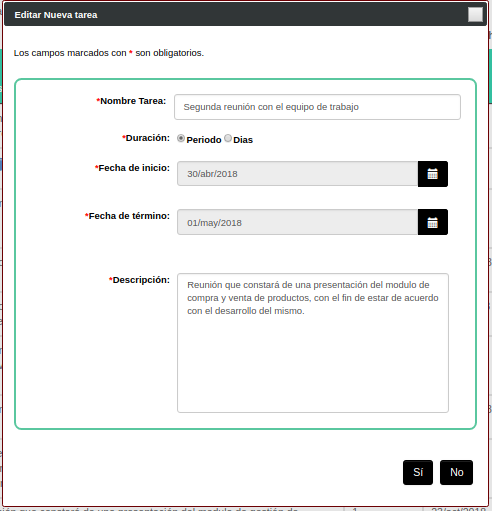
\includegraphics[width=0.8\textwidth]{./images/cu22-editar-tarea.png}
\caption{Editar tarea.} \label{fig:IU22}
\end{figure}
%===================================================================================
\subsection{CU22 Visualizar datos de la tarea}
{
\justify
\color{blue}{\textbf{Objetivo}}
}

%------------------------------------------------------------------
\justify
Permite al Lider de proyecto visualizar los datos que componen a la tarea.
%------------------------------------------------------------------
{
\justify
\color{blue}{\textbf{Diseño}}
}
%-------------------------------------------------------------------------------
\justify
En la figura \ref{fig:IU23} se muestra la pantalla, en donde permite al Lider de proyecto visualizar los datos que componen a la tarea.

\begin{figure}[htb]
\centering
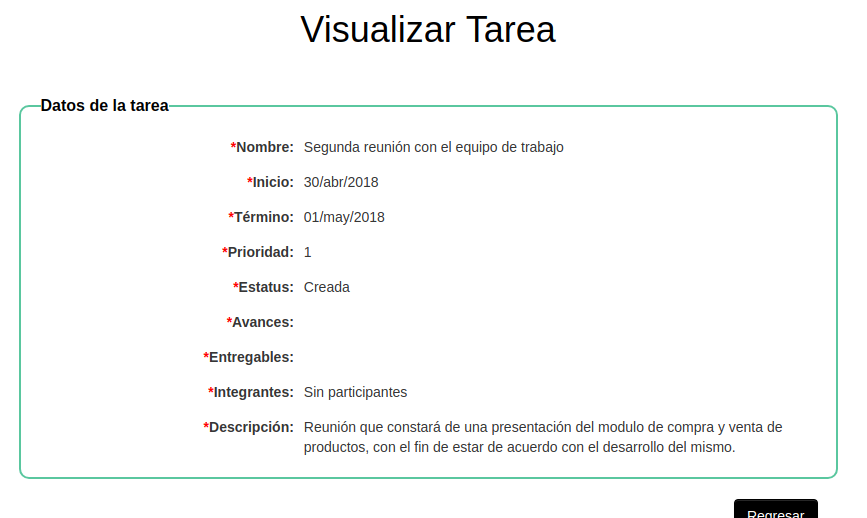
\includegraphics[width=0.8\textwidth]{./images/cu23-visualizar-datos-tarea.png}
\caption{Relacionar tareas.} \label{fig:IU23}
\end{figure}
%===================================================================================
\subsection{CU27 Ver diagrama de gantt}
{
\justify
\color{blue}{\textbf{Objetivo}}
}

%------------------------------------------------------------------
\justify
Permite al Lider de proyecto visualizar el diagrama de gantt con las tareas del proyecto.
%------------------------------------------------------------------
{
\justify
\color{blue}{\textbf{Diseño}}
}
%-------------------------------------------------------------------------------
\justify
En la figura \ref{fig:IU27} se muestra la pantalla, en donde permité al Lider de proyecto visualizar el diagrama de gantt con las tareas del proyecto.

\begin{figure}[htb]
\centering
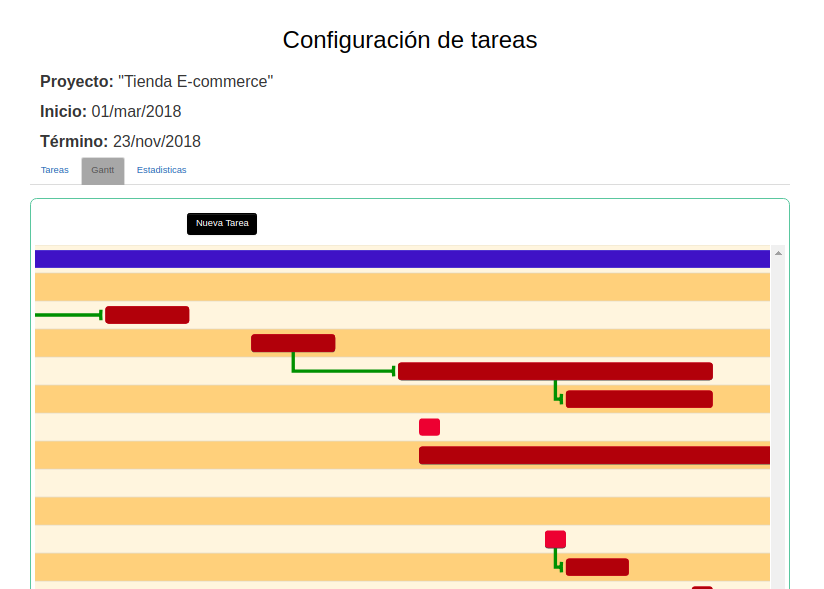
\includegraphics[width=0.8\textwidth]{./images/cu27-ver-diagrama-gantt.png}
\caption{Ver diagrama de gantt.} \label{fig:IU27}
\end{figure}
%===================================================================================
\subsection{CU28 Ver estadisticas de avances de las tareas}
{
\justify
\color{blue}{\textbf{Objetivo}}
}

%------------------------------------------------------------------
\justify
Permite al Lider de proyecto visualizar los diagramas con los reportes de avances registrados por el mismo lider así como de los colaboradores del proyecto.
%------------------------------------------------------------------
{
\justify
\color{blue}{\textbf{Diseño}}
}
%-------------------------------------------------------------------------------
\justify
En la figura \ref{fig:IU28} se muestra la pantalla, en donde permite al Lider de proyecto visualizar los diagramas con los reportes de avances registrados por el mismo lider así como de los colaboradores del proyecto..

\begin{figure}[htb]
\centering
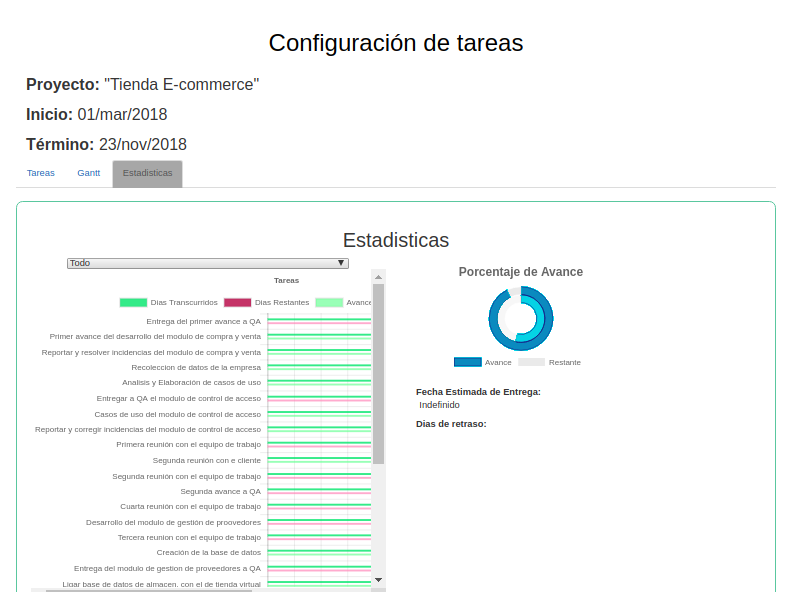
\includegraphics[width=0.8\textwidth]{./images/cu28-ver-estadisticas-avances-tareas.png}
\caption{Ver estadisticas de avances de las tareas.} \label{fig:IU28}
\end{figure}
%===================================================================================
\subsection{CU29 Mis tareas}
{
\justify
\color{blue}{\textbf{Objetivo}}
}

%------------------------------------------------------------------
\justify
Permite al Lider de proyecto y al colaborador, ver la tareas que tinen asignadas en el proyecto que estan participando.
%------------------------------------------------------------------
{
\justify
\color{blue}{\textbf{Diseño}}
}
%-------------------------------------------------------------------------------
\justify
En la figura \ref{fig:IU29} se muestra la pantalla, en donde permite al Lider de proyecto y al colaborador, ver la tareas que tinen asignadas en el proyecto que estan participando.

\begin{figure}[htb]
\centering
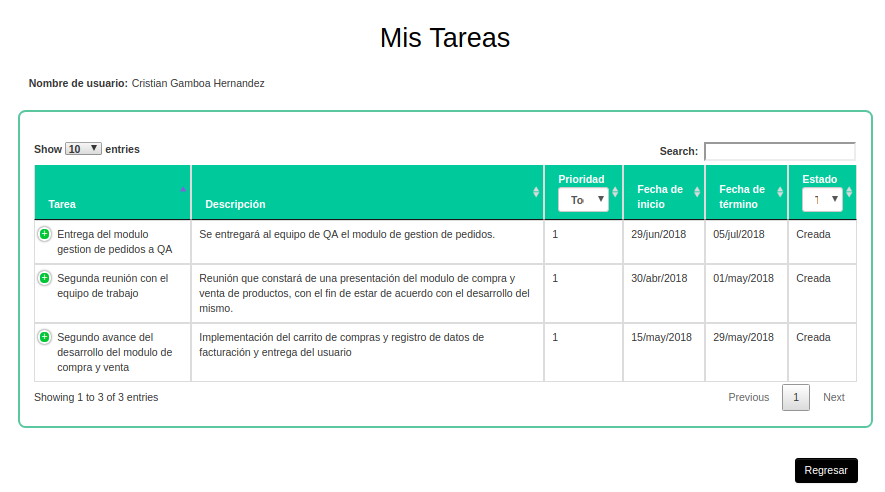
\includegraphics[width=0.8\textwidth]{./images/cu29-mis-tareas.png}
\caption{Ver estadisticas de avances de las tareas.} \label{fig:IU29}
\end{figure}

\newpage
%===================================================================================
\subsection{CU31 Ver avances commit}
{
\justify
\color{blue}{\textbf{Objetivo}}
}

%------------------------------------------------------------------
\justify
Permitir al Lider de proyecto y al colaborador, ver los detalles del avance del commit.
%------------------------------------------------------------------
{
\justify
\color{blue}{\textbf{Diseño}}
}
%-------------------------------------------------------------------------------
\justify
En la figura \ref{fig:IU31} se muestra la pantalla, en donde Permitir al Lider de proyecto y al colaborador, ver los detalles del avance del commit.

\begin{figure}[htb]
\centering
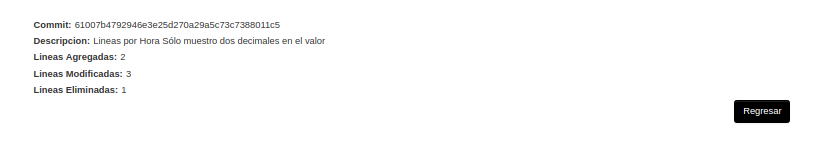
\includegraphics[width=0.8\textwidth]{./images/cu31-avance-commit.png}
\caption{Ver estadisticas de avances de las tareas.} \label{fig:IU31}
\end{figure}

\newpage